\documentclass[twocolumn,10pt]{article}

% ======================
% PACKAGES
% ======================
\usepackage[a4paper,margin=1.8cm]{geometry}
\usepackage{amsmath,amssymb}
\usepackage{graphicx}
\usepackage{float}
\usepackage{caption}
\usepackage{subcaption}
\usepackage{siunitx}
\usepackage{bm}
\usepackage{mathptmx}
\usepackage{ragged2e}  % put this in the preamble
\usepackage{titlesec}
\usepackage{authblk}

\usepackage{hyperref}
\hypersetup{
    colorlinks=true,
    linkcolor=blue,
    citecolor=blue,
    urlcolor=blue
}
%=======OUR PACKAGES================
\setlength{\columnsep}{0.6cm}
\renewcommand\thesubsubsection{\Alph{subsubsection}}
\usepackage{titlesec}

\titleformat{\section}
  {\centering\normalfont\Large\bfseries}
  {\thesection}{0.5em}{}

\titleformat{\subsection}
  {\centering\normalfont\large\bfseries}
  {\thesubsection}{0.5em}{}

\titleformat{\subsubsection}
  {\centering\normalfont\normalsize\bfseries}
  {\thesubsubsection}{0.5em}{}

%====================================

% ======================
% TITLE
% ======================
\title{\textbf{Molecular Dynamics Simulation of Argon}}
\author{Konstantinos Pourgourides$^{\dagger}$, Kyproula Mitsidi$^{\dagger}$}
\affil{\small $\dagger$ Faculty of Applied Sciences, Delft University of Technology, Lorentzweg 1, 2628 CK, Delft, The Netherlands}
\date{}

% ======================
% DOCUMENT
% ======================
\begin{document}

\twocolumn[
\maketitle
\vspace{-2.5em}
\begin{center}
\textbf{ABSTRACT}\\
\vspace{0.7\baselineskip}
\begin{minipage}{0.8\textwidth}


We present a Molecular Dynamics simulation of Argon atoms in a periodic FCC lattice using a Lennard-Jones potential. We discuss the underlying physical and mathematical mechanisms of the simulation, and perform validation checks to ensure its reliability. We explore the structure of the Pair Correlation Function for the solid, liquid and gaseous phases of Argon, and the relation between pressure and atomic density for different temperatures. Our results are in agreement with established literature, supporting the validity of our methods. Lastly, we determine the relation between the computational time and simulation time steps, as well as the rate of change of computational time with respect to the number of simulated atoms, revealing interesting findings on the computational limits of the simulation.

\end{minipage}
\end{center}
\vspace{1.5\baselineskip}
]

% ======================
\section{Introduction}
\vspace{-1em}
% ======================
Molecular Dynamics (MD) refers to a family of numerical techniques which are used to simulate the dynamical evolution of systems that contain a large number of interacting atoms  \cite{md}. The trajectories are obtained by numerical integration of Newton's equation for each atom, where interatomic forces arise as a result of potential energy.

Due to the complex nature of such many-body systems they are formidable to investigate atom-by-atom; for this reason, MD simulations mostly study macroscopic quantities which emerge from statistical averages. The averages can be taken over different microcanonical ensembles, or over time, if the system under investigation obeys the ergodic hypothesis\cite{computational_book}.

The essence of MD simulations can be captured in a few simple steps, starting from the initialization of atomic positions and velocities, which are subsequently updated over a desired amount of time in discrete time steps according to Newton's equation. Throughout this iterative process, application of boundary conditions, velocity rescaling and the calculation of physical quantities take place.

In this report, we present an MD simulation of Argon atoms in a 3 dimensional box equipped with an face centered cubic (FCC) lattice, where the dynamical evolution of the system is dictated by the Lennard-Jones potential and periodic boundary conditions. The second section deals with the methods and theory that underlie the simulation, such as the relevant physical and computational parameters, the initialization of atomic positions and velocities, the algorithm used for the time evolution of the system, and the calculation of observables and their errors. In the third section we perform some validation checks, display results concerning physical observables and how they relate to established literature, and present some findings regarding the computational performance of the simulation. In the final section, we conclude by highlighting the key results.

% ======================
\section{Methods and Theory}
% ======================

\subsection{Simulation Setup}

The simulation makes use of some tunable parameters to prepare the environment in which the atoms will exist and interact. Firstly, the simulation parameters such as the duration of a discrete time step h, the number of total time steps $N_h$ and the length of the simulation box, given in integer multiples of the lattice constant $a$, denoted as $n$. Secondly, there are the physical parameters such as the temperature $T$ of the system and the atomic density $\rho = N/V$, where $N$ is the number of atoms in the simulation and $V = (na)^3$ the volume of the box. The number of atoms is dictated by $n$, because an FCC lattice of edge length $L = na$ contains at most $4n^3$ atoms if all the sites are occupied \cite{kittel}, which is the case in this simulation.
Additionally, some physical constants are frequently used throughout for various calculations, such the mass of Argon atoms $m_A=6.63\times10^{-26}\text{kg}$ and the Boltzmann constant $k_B=1.38\times10^{-23}\text{JK}^{-1}$.\\

Lastly, some constants were used to convert the simulation to dimensionless units in the following way: $x = \tilde\alpha x^*, \ t = \tilde\beta t^*, \ m = \tilde\gamma m^*$, where $x,t$ and $m$ are the position, time and mass respectively; their starred counterparts are dimensionless. These constants were found to be $\tilde\alpha = \sigma, \ \tilde\beta = \sqrt{m\sigma^2/\varepsilon}$ and $\tilde\gamma = m$, where $\sigma = 3.41\mathrm{\AA}$ and $\varepsilon/k_B = 119.8K$.\\

Throughout the simulation, atom pairs interact with each other through the Lennard-Jones potential

\begin{equation}
    U(r) = 4\varepsilon\left[\left(\frac{\sigma}{r}\right)^{12} - \left(\frac{\sigma}{r}\right)^{6}\right]
    \label{LJ}
\end{equation}

\noindent where $r$ is the pair-wise distance between atoms. Thus, we see that $\sigma$ and $\epsilon$ are connected to $U(r)$ through

\begin{equation}
    U(\sigma) = 0, \quad \varepsilon= -U(r_{\text{min}}) \ .
\end{equation}

\noindent Evidently, $\sigma$ is the interatomic distance at which the pair-wise potential energy is zero; for $r>\sigma$ ($r<\sigma$) atoms attract (repulse) each other. Additionally, $\varepsilon$ represents the minimum interaction energy between a pair of atoms; larger (smaller) values of $\varepsilon$ correspond to stronger (weaker) attraction.\\

Combinations of these units were used throughout the simulation to simplify equations and give rise to natural units. For example, distance, energy and temperature are measured in units of $\sigma$, $\varepsilon$, and $\varepsilon k_B^{-1}$ respectively. In the observables and results sections, physical quantities are reported in their natural units, while relevant equations also display the corresponding natural units in brackets. 

\subsection{Initialization}

Before time evolution takes place, the positions $\{\mathbf{x}_i(0),\dots,\mathbf{x}_N(0) \}$ and velocities $\{\mathbf{v}_i(0),\dots,\mathbf{v}_N(0) \}$ of atoms must be initialized. The atoms are placed on the sites of an FCC lattice, and velocity components are drawn from a Gaussian distribution with the following parameters

\begin{equation}
    \mathbf{v}_i(0) \sim \mathcal{N}\left( 0,\sqrt{k_BT/m_A} \right), \ \forall i\in\{1,\dots,N\}.
    \label{gauss}
\end{equation}

\noindent The mean $\mu=0$ is such that atoms do not have a directional bias, and the standard deviation $\sigma = \sqrt{k_BT/m_A}$ originates from the equipartition theorem $\langle u_{x_i} \rangle^2 = k_BT/m_A$.\\

Even though the initial velocity components of the i$^{\text{th}}$ atom $\mathbf{v}_i(0)$ are normally distributed, its initial speed $v_i(0) = \sqrt{\mathbf{v}_i(0)\cdot\mathbf{v}_i(0)}$ follows the Maxwell-Boltzmann distribution

\begin{equation}
    P(v_i(0)) = 4\pi v_i^2(0)\left( \frac{m}{2\pi k_BT}\right)^{\frac{3}{2}} \exp\left(-\frac{m_Av_i^2(0)}{2k_BT}\right)
\end{equation}

\noindent which derives from the performance of a spherical coordinate transformation on the Gaussian joint probability density of the velocity components.

\subsection{Time Evolution}

The motion of atoms at any point in time is dictated by Newton's second law
\begin{equation}
    \mathbf{F}(\mathbf{x}_i(t)) = m_A\frac{d^2\mathbf{x}_i(t)}{dt^2}, \ \forall i\in\{1,\dots,N\}.
    \label{force}
\end{equation}

\noindent The force that each atom experiences is due to Lennard-Jones interactions with all the other atoms, and can be expressed as

\begin{equation}
    \mathbf{F}(\mathbf{x}_i(t)) = -\bm{\nabla}_iU\left( \mathbf{x}_1(t),\dots,\mathbf{x}_N(t)\right), \ \forall i\in\{1,\dots,N\}.
\end{equation}

These equations cannot be solved analytically, and thus a discrete time integration scheme is employed to numerically approximate them, known as the Velocity-Verlet algorithm.

\subsubsection{Velocity-Verlet Algorithm}

After the initialization process, the position and velocity components of each atom are updated per time step $h$ according to the Verlet algorithm \cite{verlet}
\begin{align}
   \mathbf{x}_i(t+h) &= \mathbf{x}_i(t) + h\mathbf{v}_i(t) + \frac{h^2}{2}\mathbf{F}_i(\mathbf{x}(t))
   \label{verlet1}
   \\
   \mathbf{v}_i(t+h) &= \mathbf{v}_i(t) + \frac{h}{2}\left[\mathbf{F}_i(\mathbf{x}(t)) + \mathbf{F}_i(\mathbf{x}(t+h)) \right]    
   \label{verlet2}
\end{align}

The choice of algorithm was based on the fact that it belongs to the family of so-called \textit{symplectic integrators}, which preserve the volume of phase-space as the system evolves in time.\\

To demonstrate this with a simple example, we consider a single atom moving in one dimension. The infinitesimal phase-space area taken by the canonical coordinates $(x(t),p(t))$ of the atom at a certain moment $t$ is $A(t) = dx(t)dp(t)$. At the next time step, the area will be transformed as 

\begin{equation}
    A(t+h) = \left[\det J\right] A(t), \ \text{where} \
    J = \left[ \begin{array}{c@{\hspace{0.5mm}}c}  % 10mm between columns
        \frac{\partial x(t+h)}{\partial x(t)} & \frac{\partial x(t+h)}{\partial p(t)}\\[2mm] 
        \frac{\partial p(t+h)}{\partial x(t)} & \frac{\partial p(t+h)}{\partial p(t)} 
\end{array}
\right] \ .
\end{equation}

We see that the determinant of the Jacobian acts as a scaling factor for the area. According to Eqs. (\ref{verlet1},\ref{verlet2}), $\det J = 1$, and thus the phase-space area is not distorted as the system evolves, which is a characteristic of symplectic integrators. This ensures that the energy remains bounded, leading to approximate conservation of energy over many time steps.\\

Alternative schemes such as Euler's method do not preserve the structure of phase space ($\det J_{\text{Euler}} \neq 1$) and lead to unnatural energy shifts over time. When this discussion is generalized for $N$ atoms and $d$ dimensions, equations are more complex but the essence remains the same.

\subsubsection{Boundary Conditions}

The simulation enforces periodic boundary conditions; intuitively, the atoms are forced to stay within the simulation box, where $(x_i(t),y_i(t),z_i(t)) \in [0,L] \ \forall i \in \{1,\dots,N \}$ and $\forall t \in \{1,\dots,N_h\}$. If any of their position coordinates exceed the boundary in the respective direction, it is corrected during the Velocity-Verlet algorithm. After the positions are updated, they are modified in the following way

\begin{equation}
    \mathbf{x}_i(t) \to \mathbf{x}'_i(t) = \mathbf{x}_i(t) \ \text{mod} \ L \ .
\end{equation}

\noindent This modification ensures that atoms stay within the simulation box at all times. Let's examine the cases of interest, considering that the position of an atom in a particular direction and a specific timestep can be expressed as $\mathbf{x}_i(t) = cL, \ c>0$

\begin{equation}
    cL \ \text{mod} \ L =
    \begin{cases}
        cL, \ &0<c<1 \\
        0, \  &c=1\\
        rL, \ &c = 1 + r
    \end{cases}
\end{equation}

\noindent where $r\in(0,1)$. An atom remains in the box if it is already in a valid position, and it is moved at 0 when it exactly reaches $L$. More interestingly, when the position of an atom is $L(1 + r)$, it is moved to $rL$, thus returning inside the box.\\

\subsubsection{Minimal Image Convention}

The periodic boundary conditions also affect the calculation of interatomic forces, as they involve the Lennard Jones potential, which depends on the pair-wise distances between atoms. When the force on atom $i$ from atom $j$ is calculated, their pair-wise distance $r_{ij} = \sqrt{(x_i-x_j)^2+(y_i-y_j)^2+(z_i-z_j)^2}$ needs to conform to the periodic boundary conditions, and thus coordinates of atom $j$ might need adjustment. For each coordinate, one of these adjustments is made

\begin{equation}
    x_j' = 
    \begin{cases}
        x_j, \quad  &-L/2 < x_i - x_j < L/2 \\
        x_j + L, \ &x_i - x_j > L/2 \\
        x_j - L, &x_i-x_j < -L/2 
    \end{cases}
\end{equation}

\noindent and similarly for $y_j'$ and $z_j'$. The pair-wise distance is minimal when calculated using the image of atom $j$ at $(x_j',y_j',z_j')$, and hence the name \textit{minimal image convention}.

\subsubsection{Velocity Rescaling}

While we want to simulate Argon atoms at a desired target temperature $T_{\text{target}}$, this is not simply achieved by initializing the velocities according to a Gaussian distribution with $\sigma = \sqrt{k_BT_{\text{target}}/m_A}$ (Eq. \eqref{gauss}). In reality, the temperature is a kinetic variable, meaning that it is defined at every time step through the kinetic energy of the system

\begin{equation}
    T(t) = \frac{m_A}{3N_{\text{dof}}k_B}\sum_i^N|\mathbf{v}_i(t)|^2
\end{equation}

\noindent where $N_{\text{dof}} = N-1$. Because of unpredictable interactions between atoms, the kinetic energy might account for a different temperature than $T_{\text{target}}$. If this is not forcefully corrected, $T(t)$ will drift off completely as time evolves. To alleviate this inconsistency, velocity rescaling is needed.\\

If the velocities of atoms, and thus the kinetic energy at a certain time step accounts for a different temperature than $T_{\text{target}}$, they are rescaled to correspond to the kinetic energy that would correctly produce $T_{\text{target}}$ in the following way

\begin{equation}
    \mathbf{v}_i(t) \to \mathbf{v}_i'(t) = \left(\frac{T_{\text{target}}}{T(t)}\right)^{\frac{1}{2}}\mathbf{v}_i(t) = \left(\frac{3N_{\text{dof}} \ k_BT_{\text{target}}}{m_A\sum_j^N|\mathbf{v}_j(t)|^2}\right)^{\frac{1}{2}} \mathbf{v}_i(t) \ .
\end{equation}

Rescaling is forced periodically during time evolution every $n_{\text{rescale}}$ time steps, and stops when $|T(t)-T_{\text{target}}| < \zeta$ is achieved for more than $n_{\text{force}}$ consecutive time steps. The threshold $\zeta$, $n_{\text{rescale}}$ and $n_{\text{force}}$ are all tunable parameters. The last time step in which velocity rescaling takes place is denoted by $t_{\text{lrs}}$.

\subsection{Observables}

As explained in the introductory section, observables are calculated as averages over time, where we only use time steps $t>t_{\text{lrs}}$, when the system is considered to be in equilibrium

\begin{equation}
    \langle A\rangle = \frac{1}{N_h-t_{\text{lrs}}}\sum_{i = t_{\text{lrs}}}^{N_h}A_i
    \label{time avg}
\end{equation}

In this report, we will investigate two observables. Firstly, we will study the Pair Correlation Function $g(r)$ and its revelations on the spatial structure of Argon. Secondly, we will study pressure $P$ and how it is affected by atomic density $\rho$ and temperature $T$.

\subsubsection{Pair Correlation Function}
 Pair Correlation Function (PCF) $g(r)$, also known as radial distribution function, measures the probability of observing an atom at distance $r$ from another atom relative to the probability expected for an ideal gas \cite{Rahman}. PCF is calculated by counting all atoms n(r) that are separated by distances within $[r,r+\Delta r]$, where $\Delta r$ is the width of the spherical shell. The above is expressed by
\begin{equation}
    g(r) = \frac{2V}{N(N-1)} \frac{\langle n(r) \rangle}{4 \pi r^2 \Delta r} 
    \label{g}
\end{equation}
where $2V/N(N-1)$ normalizes the probability density with respect to the ideal gas. The distribution comes in distinct forms for different states of matter, which will be explored in this report.\\
 
 Generally, in solids, the atoms vibrate around fixed lattice positions and are arranged in a highly ordered structure. It is expected to observe pronounced peaks at characteristic distances determined by the crystal lattice. The $i^{th}$ peak corresponds to the $i^{th}$ coordination shell with an amplitude proportional to the number of neighbors in that shell. Specifically, these peaks are expected to be found at distances $a/\sqrt{2}, \  a, \ \sqrt{3}a/\sqrt{2}$ and so on \cite{kittel}. \\

The number of neighbors for each atom in a coordination shell is given by integrating the PCF across the corresponding peak 

\begin{equation}
      n_{\text{shell}} = 4\pi\Delta r \int_{r_0}^{r_f}r^2g(r) dr \ .
      \label{nshell}
\end{equation}

\noindent where $r_f -r_0$ is the width of the peak. In an FCC lattice, the expected number of neighbors for the first three coordination shells is 12, 6 and 24  \cite{chandler}.\\


In contrast, liquids are dynamic and packed more loosely. Consequently, the probability of observing pair-wise distances between peaks is higher, making them less pronounced. The first coordination sphere is expected around $\sigma$, containing the most atoms, making it the most prominent peak. A decrease follows this peak, as repulsive interactions reduce the probability of observing atoms in this region. The following peaks occur in irregular intervals as atoms diffuse in the liquid, resulting in the loss of long-range structure as interactions become negligible, $g(r) \approx 1$. \\

In gases, atoms do not follow a regular structure, which is manifested in the broadened peaks of the PCF, expected to take these values

\begin{equation}
     \begin{cases}
        g(r) = 1, &\quad r>2\sigma\\
        g(r)>1, &\quad \sigma<r<2\sigma\\
        g(r)=0, &\quad r<\sigma
    \end{cases}
\end{equation}

\noindent The above can be explained rather simply by taking into consideration the effect of Lennard-Jones potential. The first case refers to atoms with pair-wise distances such that their mutual attraction becomes negligible. Consequently, the system adopts an ideal-gas-like behavior where no interactions are present, and thus $g(r)\approx 1$. The second case corresponds to pair-wise distances where the mutual attraction is effective, thus making it more probable to find atoms there, $g(r)>1$. The last case refers to the repulsive regime of the potential, and such configurations are highly unlikely, $g(r)\approx 0$.
 
\subsubsection{Pressure}
We aim to investigate the well-known macroscopic observable of pressure, and to perform the necessary calculations we make use of the following formula, which utilizes the Virial theorem 

\begin{equation}
    \frac{\beta P}{\rho} = 1 - \frac{\beta}{3 N} \left<\frac{1}{2} \sum_{i,j} r_{ij} \frac{\partial U}{\partial r_{ij}} \right> \quad \left[\varepsilon\sigma^{-3}\right]
    \label{virial}
\end{equation}
where $\beta=1/k_BT$, and $r_{ij}$ is the pair-wise distance between atoms. The left-hand side of Eq. \eqref{virial} represents the pressure in natural units.\\

We will study changes in pressure as a function of atomic density $\rho$ for fixed values of temperatures. From low to moderate densities, atoms are not closely packed together and we expect interatomic attractions to dominate the landscape, leading to a minimum in pressure for low temperatures. For higher temperatures, the minimum becomes less pronounced or manifests itself as a plateau. As density continues to increase, we expect the atoms to come closer together, resulting in large repulsive forces, and a steady increase in pressure.\\

Pressure can take both positive and negative values depending on whether the interactions are dominated by attractive or repulsive forces. If the system tends to contract, then the pressure is negative, and if it tends to expand, the pressure is positive.
\subsection{ Errors }

In this report, we will estimate the errors of the observables using the autocorrelation function \cite{computational_book} and error propagation.

\subsubsection{Autocorrelation Function} 
The error of the quantity in Eq. \eqref{time avg} cannot be estimated using the well-known formula for the standard deviation
\begin{equation}
 \sigma_A = \sqrt{\frac{1}{N-1}\sum_n\left(A_n - \langle A \rangle \right)^2},
\end{equation}
as the data we obtain in the simulation are correlated; The state of the system in a time step depends on the previous. To obtain a statistically uncorrelated dataset we use the autocorrelation function, defined as

\begin{equation}
\chi_A(t) =
\frac{\langle A_n A_{n+t} \rangle - \langle A_n \rangle \langle A_{n+t} \rangle}
{\sqrt{ \left(  \langle A_n^2 \rangle - \langle A_n \rangle^2\right)\times \left( \langle A_{n+t}^2 \rangle - \langle A_{n+t} \rangle^2\right)}}
\end{equation}
with 
\begin{equation}
    \langle A_n \rangle \equiv \frac{1}{N-t} \sum_{n=1}^{N-t} A_n
\end{equation}

The autocorrelation function exhibits an exponential decay $e^{-t/\tau}$, where $\tau$ is the correlation time, i.e. the least number of time steps one would have to skip to obtain uncorrelated data. By fitting the decay, we can determine $\tau$ and then calculate the error of our observable as

\begin{equation}
    \sigma_A = \sqrt{\frac{2 \tau}{N} \left(\langle A^2 \rangle - \langle A \rangle^2\right)} \ .
\end{equation}



\subsubsection{Error Propagation}
% ======================
The observables we want to investigate are functions of other variables $x_i$, and it is more efficient to compute the time averages of these variables rather than those of the observables directly. Consequently, we have to propagate the error from these variables (estimated through the autocorrelation function), to the error of the observable by applying the following formula

\begin{equation}
\sigma_{A} = \sqrt{\sum_i
\left( \frac{\partial A}{\partial x_i} \sigma_{x_i}\right)^2 
} + 2\sum_{i<j}\frac{\partial A}{\partial x_i}\frac{\partial A}{\partial x_j}\text{cov}(x_i,x_j)
.
\end{equation}

Since our observables (Eqs. (\ref{g},\ref{virial})) depend only on one variable (the time-averaged terms), the above formula reduces to

\begin{equation}
    \sigma_A = \frac{\partial A}{\partial x}\sigma_x \ .
\end{equation}

\section{Results}
% ======================
In this section, we will display our results regarding validation checks, observables and simulation performance. 

\subsection{Validation Checks}

We perform some validation checks on the initialization of positions and velocities, as well as time evolution, to ensure that the simulation works as intended. 

\subsubsection{Initialization}

The atomic positions are initialized on the sites of an FCC lattice. An example including nearest-neighbor bonds\footnote{This part was implemented with assistance from AI for visual clarity.} is displayed in Fig. (\ref{FCC}), viewed from different orientations, confirming the FCC lattice structure. 

\begin{figure}[H]
    \centering
    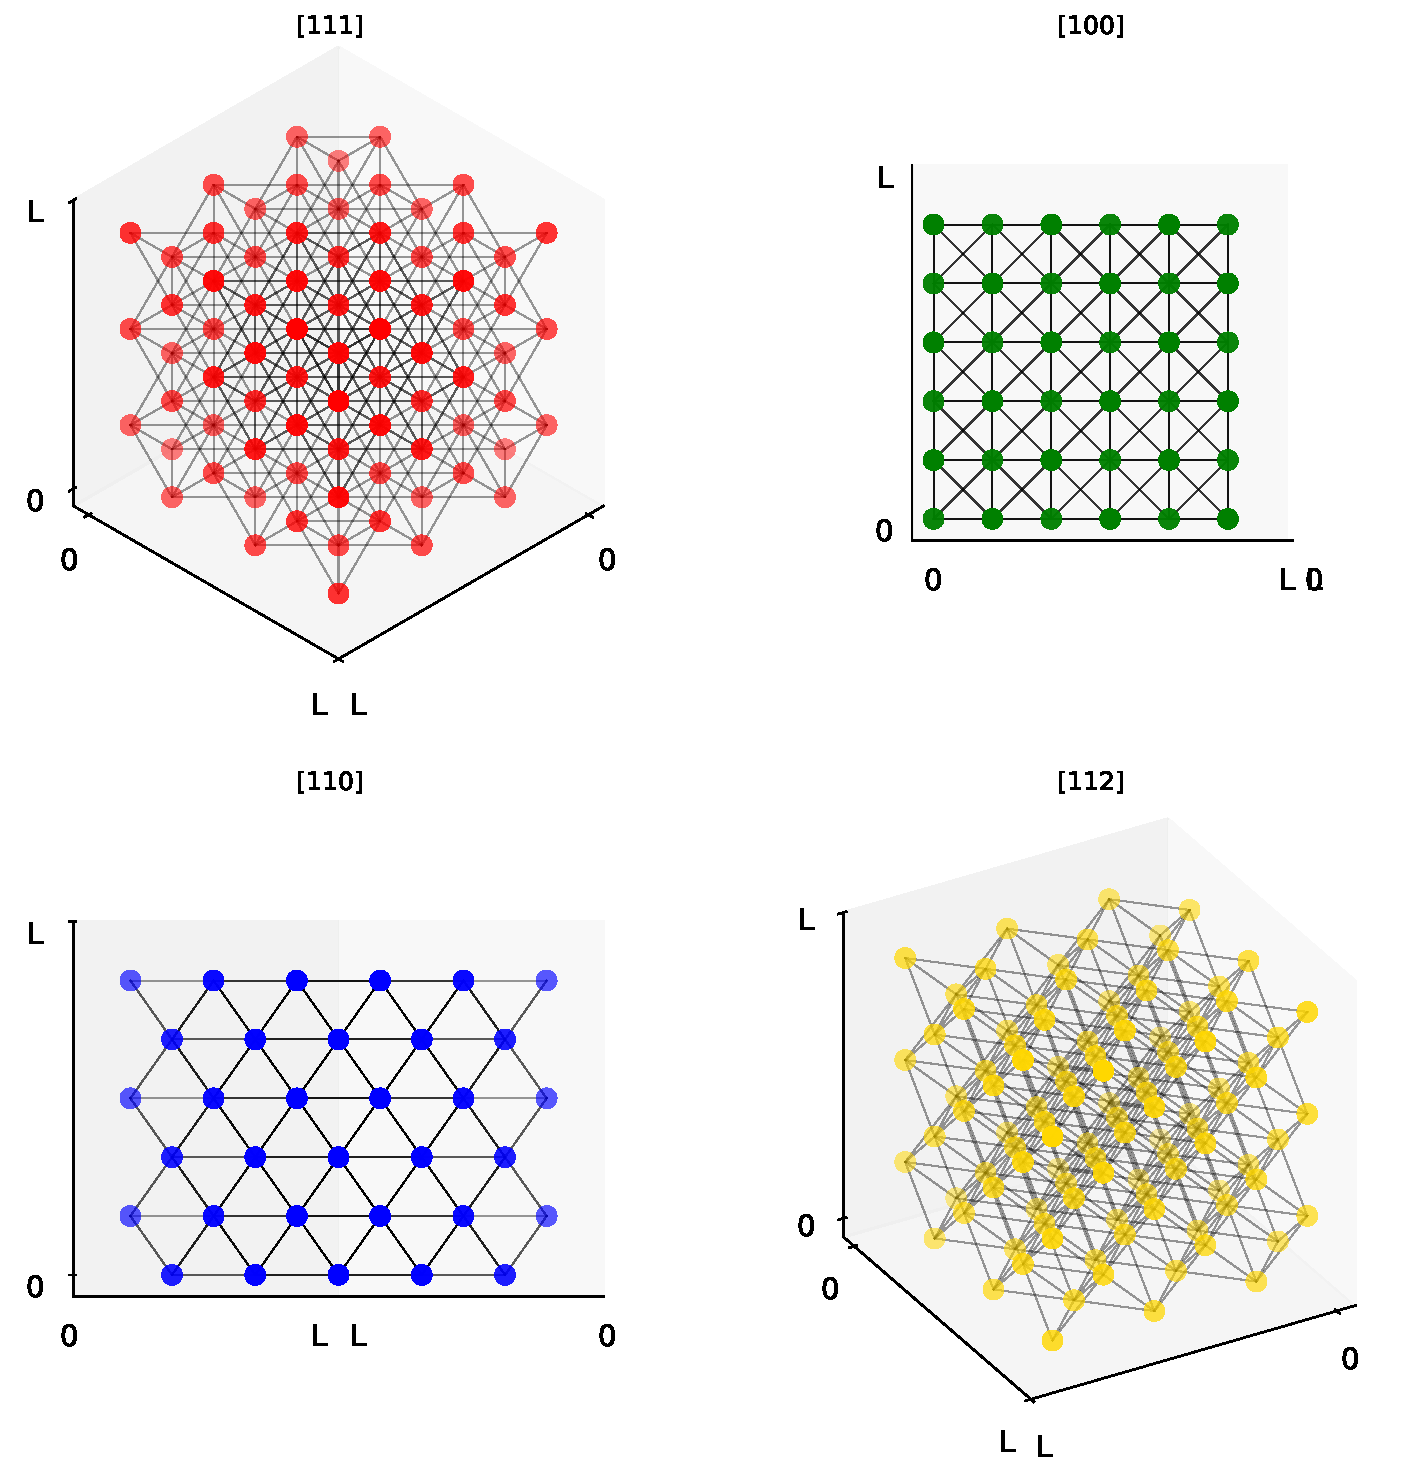
\includegraphics[width=\columnwidth]{plots/fcc.pdf}
    \caption{Four different views of the initial atomc positions on the FCC lattice for $N,\rho = \{108, 0.8 \sigma^{-3} \}$ including the nearest-neighbor bonds. The views correspond to the Miller indices \textbf{[111]} (top-left), \textbf{[100]} (top-right), \textbf{[110]} (bottom-left), and \textbf{[112]} (bottom-right).}
    \label{FCC}
\end{figure}


Additionally, we display an example of the normalized distribution of initial speeds in Fig. (\ref{maxwellboltzmann})

\begin{figure}[H]
    \centering
    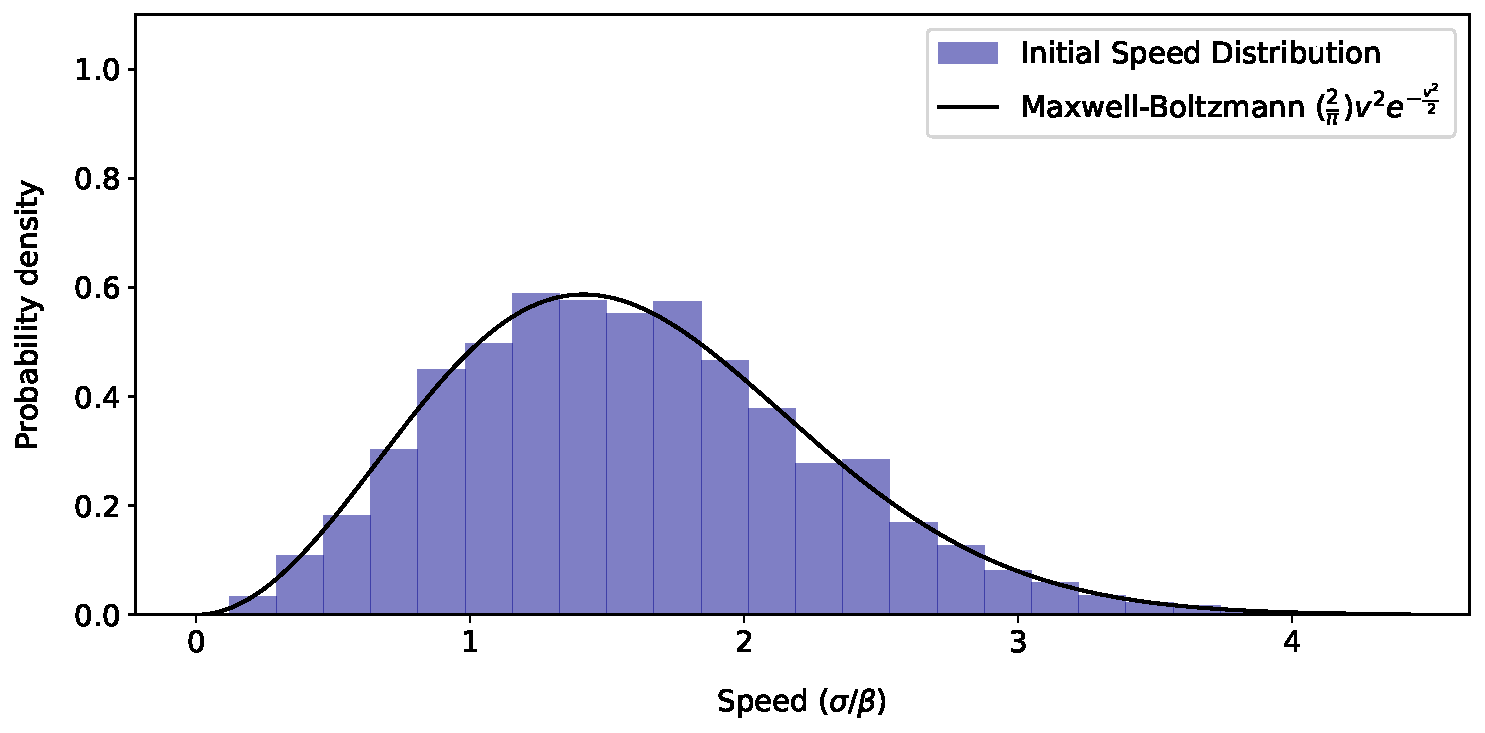
\includegraphics[width=\columnwidth]{plots/maxwell.pdf}
    \caption{Histogram of initial speeds for $N,\rho,T_{\text{target}} = \{4000, 0.8 \sigma^{-3},1 \varepsilon k_B^{-1}\}$ alongside the theoretical Maxwell-Boltzmann distribution.}
    \label{maxwellboltzmann}
\end{figure}

Evidently, there is agreement between the theoretical curve and simulation data to a large degree. Thus, we conclude that our simulation initializes positions and velocities as intended.

\subsubsection{Time evolution}

A useful validation check we can perform regarding the correct time evolution of the simulation, is to study how $T(t)$ evolves in time. We expect that prior to the last rescaling step $t_{\text{lrs}}$ the temperature is periodically forced to the exact value of $T_{\text{target}}$, and that after the rescaling process is over, $T(t)$ fluctuates around that value.\\

We display an example of temperature rescaling in Fig. (\ref{temperature}). Indeed, the temperature is abruptly forced to the target value periodically until it is stabilized, and then continues to fluctuate around that value until the end of the simulation.

\begin{figure}[H]
    \centering
    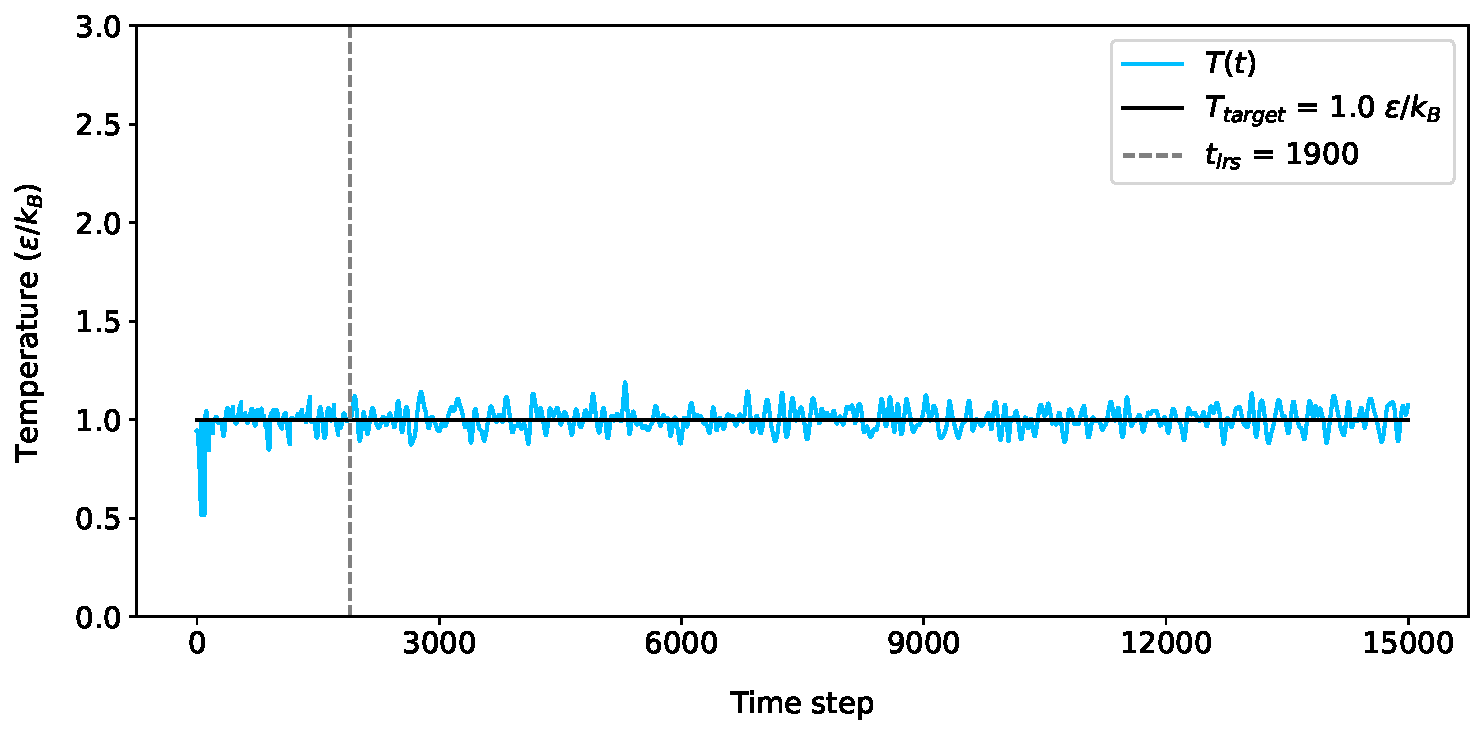
\includegraphics[width=\columnwidth]{plots/temperature.pdf}
    \caption{Temperature as a function of time step illustrating the rescaling process for $N,\rho,T_{\text{target}}, N_h,n_{\text{rescale}},n_{\text{force}},\zeta = \{108,1\sigma^{-3},1\varepsilon k_B^{-1},15000,50,150,0.05\varepsilon k_B^{-1} \}$.}
    \label{temperature}
\end{figure}

Another useful validation check is the conservation of energy. We expect the kinetic, potential and total energy to change abruptly during the initial time steps of the simulation, but to gradually stabilize until the rescaling process is completed. Then, we expect the total energy to be approximately constant, while kinetic and potential energies are symmetrically exchanged between the atoms.\\

The time evolutions of kinetic, potential and total energies per atom are illustrated in Fig. (\ref{energy}) for the same simulation run as for Fig. (\ref{temperature}). We can qualitatively see that total energy is approximately conserved.

\begin{figure}[H]
    \centering
    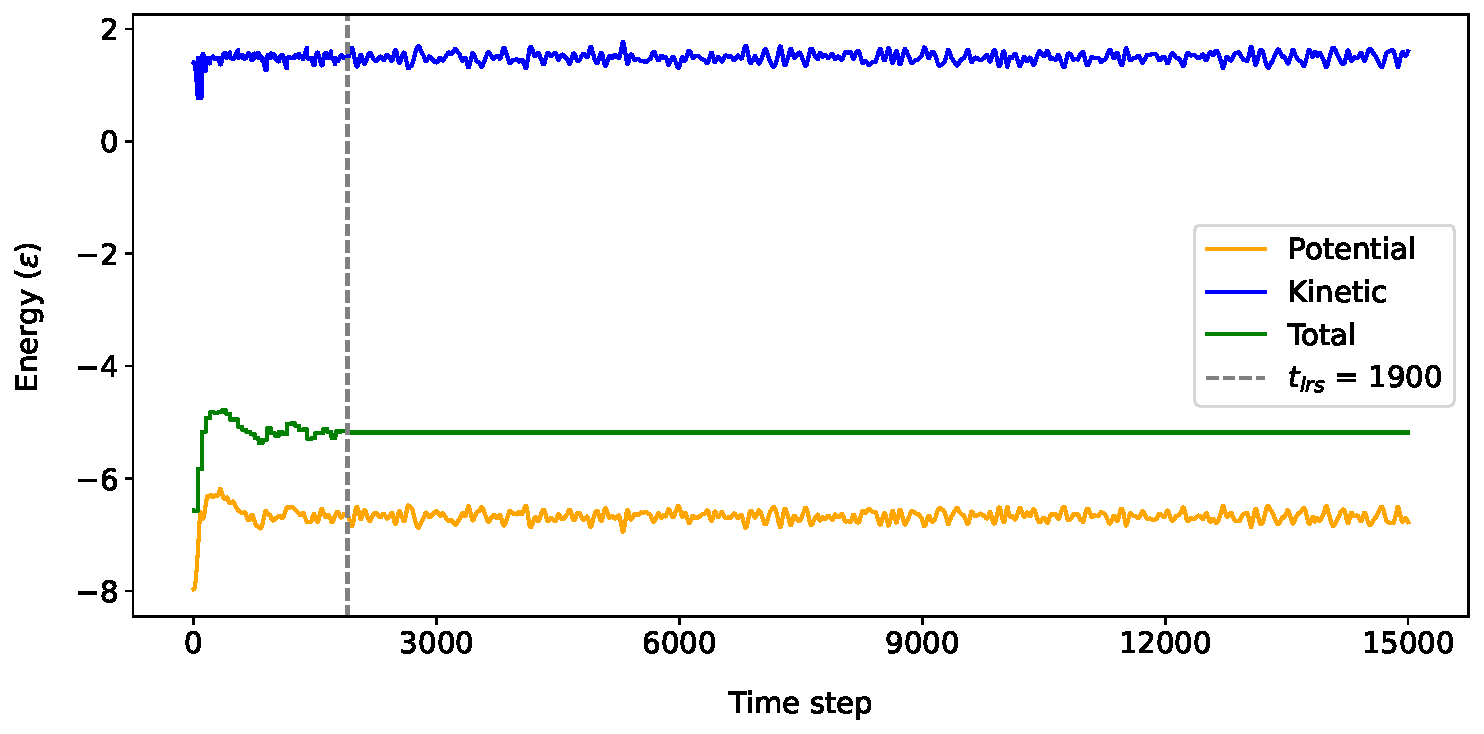
\includegraphics[width=\columnwidth]{plots/energy.pdf}
    \caption{Kinetic, potential and total energy as a function of time step for $N,\rho,T_{\text{target}}, N_h, n_{\text{rescale}},n_{\text{force}},\zeta = \{108,1\sigma^{-3},1\varepsilon k_B^{-1},15000,50,150,0.05\varepsilon k_B^{-1} \}$.}
    \label{energy}
\end{figure}

We can perform a more quantitative analysis on energy conservation by examining kinetic energy more closely, which is the only one with a predictable value. From the equipartition theorem, we know that the kinetic energy per atom should $E_{\text{kin}} = 3k_B T_{\text{target}}/2 = 1.5\varepsilon$. For our simulation, we calculate the time averaged kinetic energy to be $\langle E_{\text{kin}}\rangle = (1.481 \pm 0.086)\varepsilon $, which has a percentage error $100|\langle E_{\text{kin}}\rangle - E_{\text{kin}}|/E_{\text{kin}}$ of  $1.27\%$ and a standardized residual $|\langle E_{\text{kin}}\rangle - E_{\text{kin}}|/\sigma_{\langle E_{\text{kin}}\rangle}$ of $0.22\sigma$ away from the theoretical value, proving the approximate conservation of energy.

%temp rescaling, energies, compare with thermodynamics theory result


\subsection{Observables}
Our next step is to use the data from our simulation to investigate the observables described in the corresponding section.

\subsubsection{Pair correlation function}
To study the behavior of the PCF we ran three different simulations corresponding to the different states of matter for Argon. The temperature and density was tuned for each case to match the desired phase, as depicted in Fig. (\ref{g}). For higher temperatures, the interactions become more chaotic as atoms fluctuate strongly throughout the available space. Consequently, a lower atomic density is required to prevent the system from being dominated by repulsive interactions.

\begin{figure}[H]
    \centering
    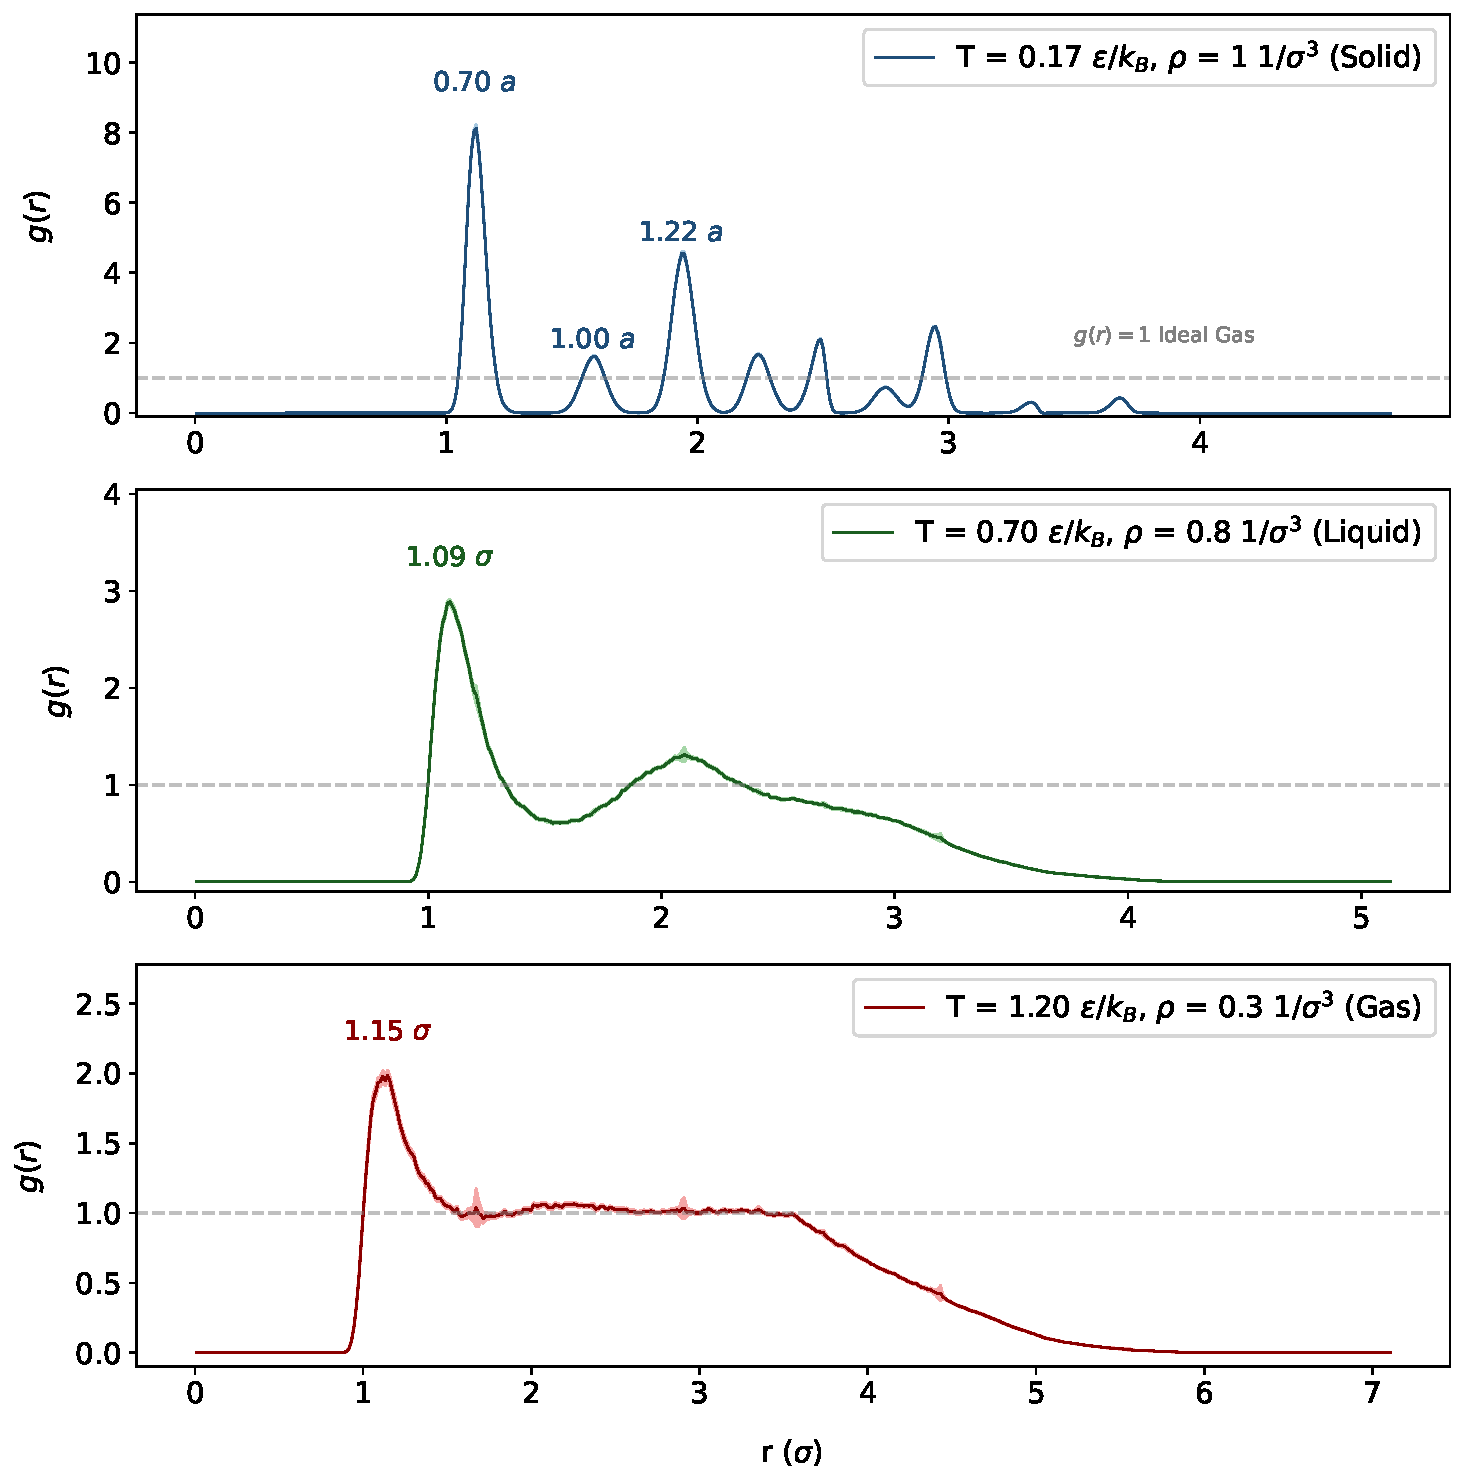
\includegraphics[width=\columnwidth]{plots/pcf.pdf}
    \caption{PCF as a function of pair-wise distance for three different sets of $(T,\rho)$ corresponding to the solid (upper), liquid (middle) and gaseous (lower) phase of Argon. The peaks are labeled by the corresponding value of $r$ in terms of the lattice constant $a$ (upper) or $\sigma$ (middle, lower) for $N, N_h,n_{\text{rescale}},n_{\text{force}},\zeta = \{108,15000,50,150,0.05\varepsilon k_B^{-1} \}$.}
    \label{g}
\end{figure}

The upper plot of Fig. (\ref{g}) is the distribution of PCF for the solid state. We observe sharp distinct peaks at different pair-wise distances, with the first three being at 0.70$a$, 1.00$a$ and 1.22$a$. These values correspond to the theoretical predictions for an FCC lattice \cite{kittel}. For this case, we can proceed with the calculation of the number of nearest neighbors in these coordination shells. Performing the calculation of Eq. \eqref{nshell}, we find the results presented in Table (\ref{coord shell}), once again validating the FCC structure \cite{chandler}.

\begin{table}[h]
    \centering
    \begin{tabular}{|c|c|c|c|}
    \hline
        Shell & Theoretical FCC  & Computational & Error (\%) \\
      \hline 
      \hline
        1 & 12 & 12.09 $\pm$ 0.02 & 0.75\\
       2 & 6 & 5.98 $\pm$ 0.02 & 0.33\\
       3 & 24 & 24.29 $\pm$ 0.05 & 1.21\\
       \hline
    \end{tabular}
    \caption{Theoretical and computational shell coordination numbers and the percentage error between them.}
    \label{coord shell}
\end{table}

The middle plot shows the PCF of Argon in the liquid phase. There is a peak at 1.09$\sigma$, relatively broader than the peaks of the upper plot, followed by a local minimum and an overall loss of long-range structure. Our results align with the theoretical predictions for liquids.\\

The upper plot illustrates the PCF of Argon in its gaseous phase. The first peak appears at 1.15 $\sigma$. For distances greater than $2\sigma$, the pair correlation function rests around the ideal gas limit, $g(r) \approx 1$; for distances less than $\sigma$, the PCF is zero, and for intermediate distances the PCF is greater than one. These results are in accordance with the expected behavior for gases.\\

Comparing these three plots, we can make several important remarks. Increase in temperature provides atoms with sufficient energy to break local bonds and fluctuate more freely. This effect is represented in the middle and lower plots by broader, less pronounced peaks, as atoms are no longer confined to well-defined positions as in the solid phase. This effect is more visible in the gaseous state, where the distribution becomes nearly uniform after $2\sigma$. Additionally, we note that the rise of temperature reduces the effectiveness of interatomic interactions, causing the system to behave more like an ideal gas. Finally, in all three plots, the PCF decays for large values of $r$, as the minimal image convention prevents such pair-wise distances from occurring.


\subsubsection{Pressure}

We studied pressure as a function of atomic density for 3 fixed temperatures which correspond to those used by Verlet in his original paper on Lennard-Jones fluids \cite{verlet} for direct comparison. Our results are depicted in Fig. (\ref{pressure}).

\begin{figure}[H]
    \centering
    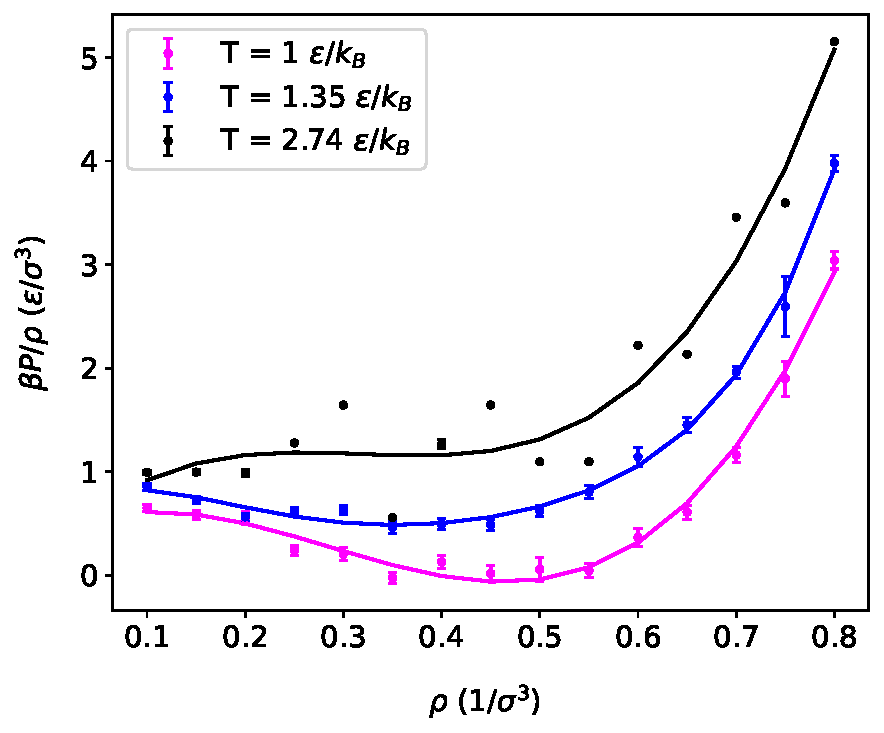
\includegraphics[width=\columnwidth]{plots/pressure.pdf}
    \caption{Pressure as a function of atomic density for 3 fixed temperatures and $N, N_h,n_{\text{rescale}},n_{\text{force}},\zeta = \{32,15000,50,150,0.05\varepsilon k_B^{-1} \}$. }
    \label{pressure}
\end{figure}

The behavior is on par with our expectations: for the low temperature, pressure is locally minimized; for the moderate temperature the minimum is less pronounced, and for the higher temperature we observe a plateau. All 3 rise monotonically for higher density values. Moreover, we performed a non-parametric fit on the data points, and a comparison with Ref. \cite{verlet} confirms that the shape of the curves is largely similar. Differences might have occurred to due different number of atoms, simulation time, and Verlet's pressure definition which includes an extra term with respect to ours. 

\subsection{Simulation Performance}

To explore the computational limits of our simulation, we performed runs for different numbers of atoms and total time steps with all other parameters fixed\footnote{These parameters include temperature and density, which do not affect the simulation time.}, and recorded the computational time for a given set of $N$ and $N_h$. The results are depicted in Fig. (\ref{performance}).

\begin{figure}[H]
    \centering
    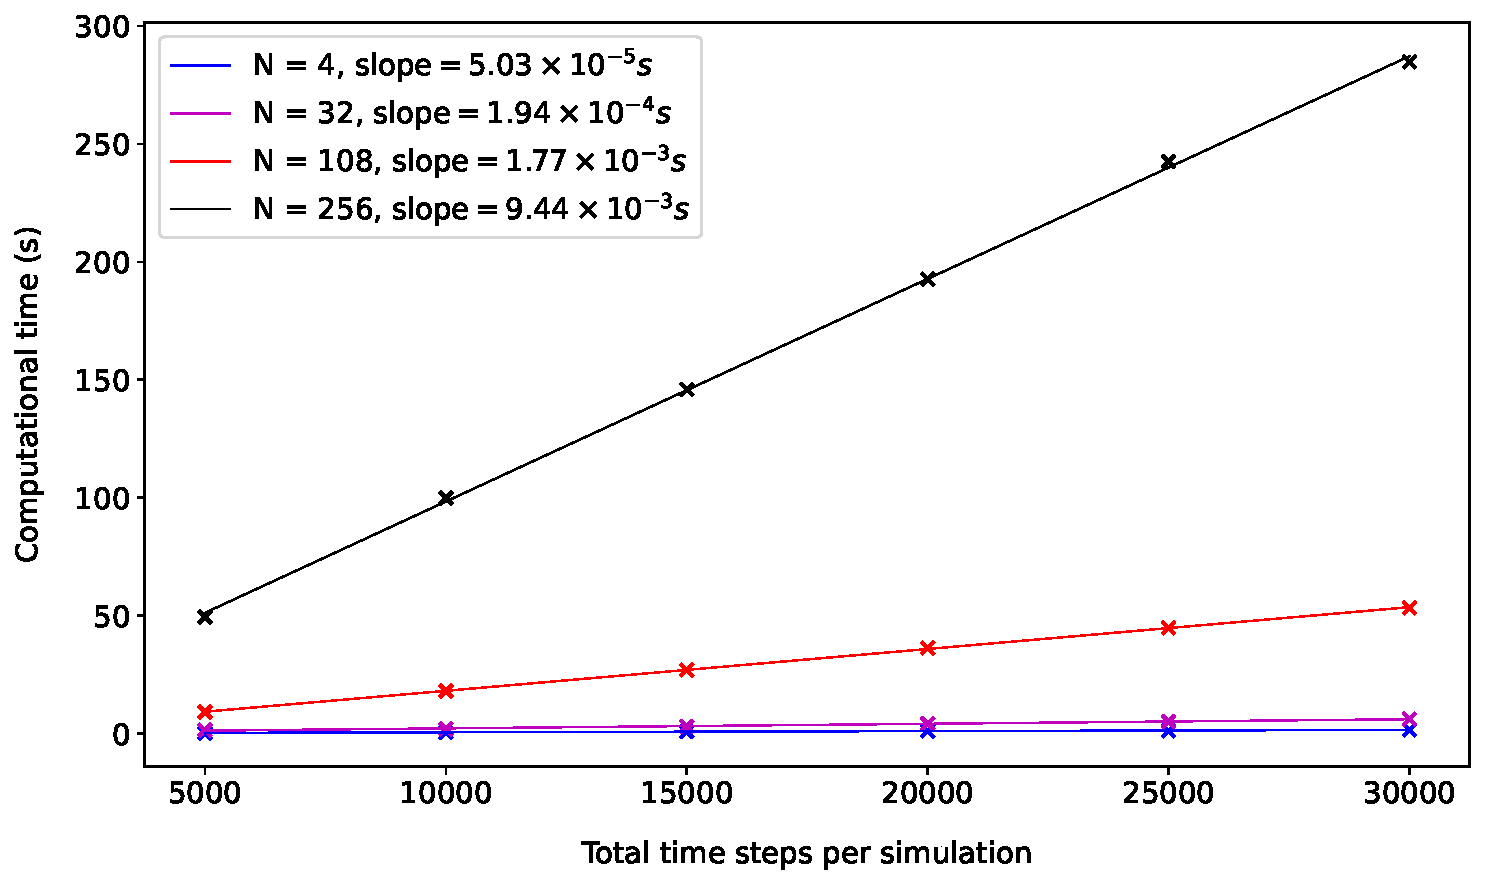
\includegraphics[width=\columnwidth]{plots/performance.pdf}
    \caption{Computational time for different values of $N$ as a function of the total number of time steps for separate simulation runs.}
    \label{performance}
\end{figure}

We observe that for a specific $N$, the growth of computational time is linearly proportional to $N_h$. The slope of each line corresponds to the following

\begin{equation*}
    \text{slope = } \frac{\Delta(\text{computational time})}{\Delta N_h} \quad [\text{s}]
\end{equation*}

Interestingly enough, when going from $N=4$ to $N=256$, the slope has a 2 orders of magnitude increase. This raises a question on the relation between the slope and $N$, which was explored, and the answer is illustrated in Fig. (\ref{slope}).

\begin{figure}[H]
    \centering
    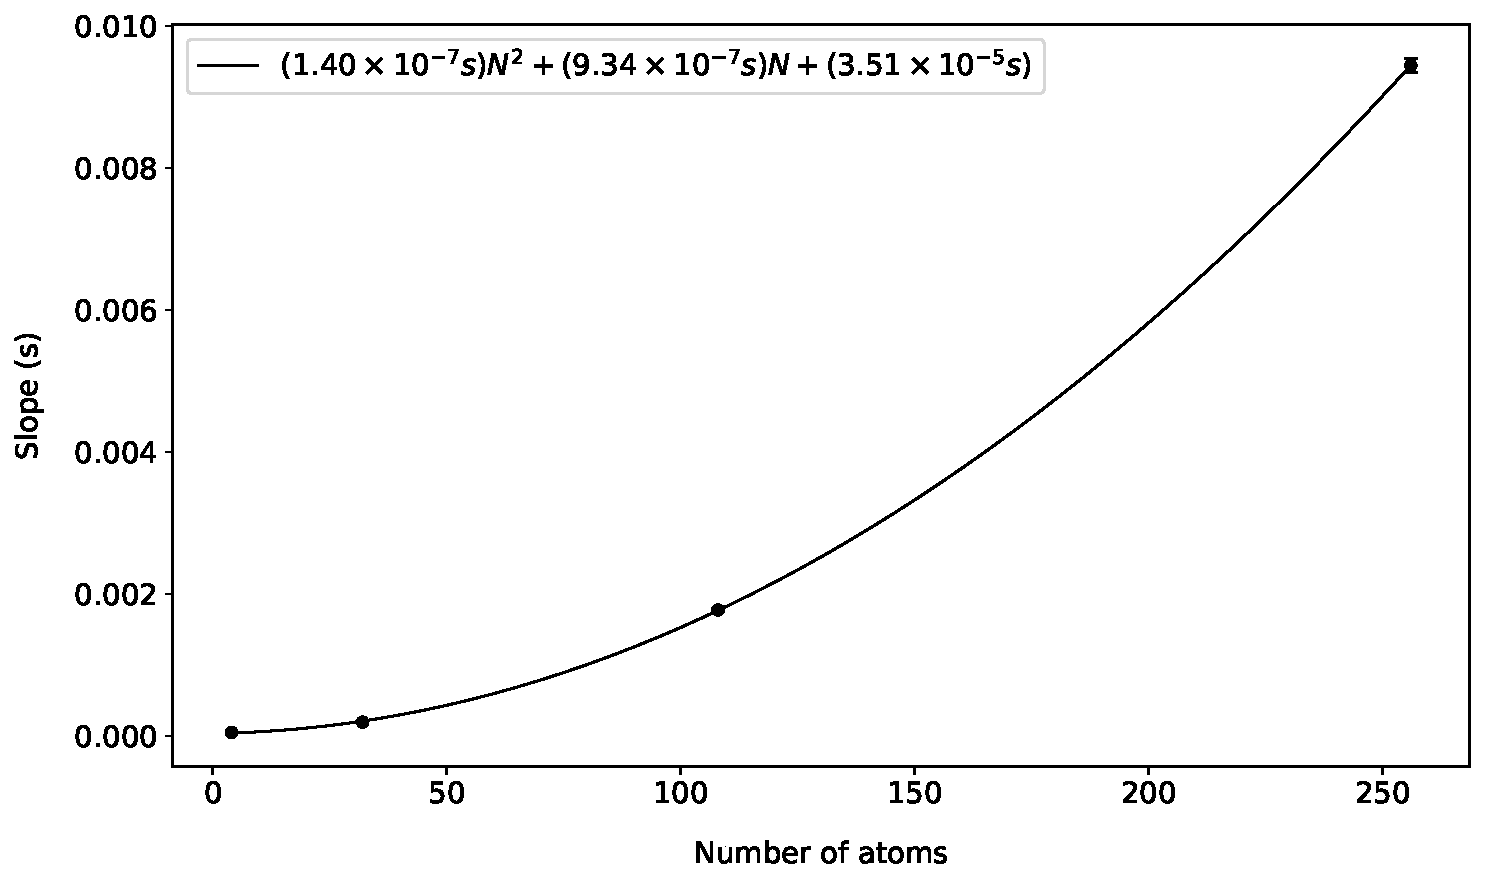
\includegraphics[width=\columnwidth]{plots/quadratic fit.pdf}
    \caption{The rate of change of computational time with respect to  $N_h$ as a function of $N$.}
    \label{slope}
\end{figure}

We observe the following relation between the quantities of interest

\begin{equation*}
        \frac{\Delta(\text{computational time})}{\Delta N_h} (N) = aN^2 + bN + c
\end{equation*}

Qualitatively, pair-wise interactions between atoms require $N(N-1) \sim \mathcal{O}(N^2)$ calculations, and the integration of position and velocities require $N \sim \mathcal{O}(N)$ calculations. The constant term derives from language-related processes that do not depend on $N$.\\

In general, the simulation can reasonably handle scenarios for up to $N=256$ for several thousand time steps, which allowed us to perform all necessary calculations regarding this report with ease. The simulation still runs, but struggles for values $N=500$ and $N=864$ even for a moderate number of time steps. For $N\geq1372$, the computational time becomes unreasonably large.\\

We would like to highlight the importance of the preceding section, as computational limitations often played a role in the physics of the simulation. In general, we noticed that larger values of $N$ lead to better alignment with theoretical expectations, and enhanced the visual representations of the system. Additionally, since we are averaging physical quantities over time, a larger number of time steps $N_h$ always reduced statistical fluctuations. For these reasons, it is essential for the simulation to support large numbers of atoms for sufficiently long time scales.

% ======================
\section{Conclusions}
% ======================

In summary, we presented a molecular dynamics simulation for Argon atoms by highlighting the relevant methods and theory underlying the setup, initializations, and time-evolution. We extensively discussed the physics and expected behavior of two relevant observables, the Pair Correlation Function and Pressure, within our simulation. The computational results are in large agreement with established literature, supporting the validity of our implementation. Additionally, we made a brief statement on the estimation and propagation of statistical errors, and performed some validation checks to ensure that the simulation works reliably. Lastly, we explored the limitations of our simulation and presented interesting findings on how the computational time scales with the number of atoms and number of time steps, providing insights on how computational limitations can manifest in the physics of the simulation. 

% ======================
\bibliographystyle{unsrt}
\bibliography{references}
% ======================

\end{document}

\begin{figure}[H]
    \centering
    \includegraphics[width=\columnwidth]{}
    \caption{Mean squared displacement as a function of lag time.}
\end{figure}

